
\bta{2009}




\section{Use of English}

\noindent
\textbf{Directions:}\\
Read the following text. Choose the best word (s) for each numbered blank
and mark A, B, C or D on ANSWER SHEET 1. (10 points)




\TiGanSpace


Research on animal intelligence always makes me wonder just how smart
humans are. \cloze the fruit-fly experiments described by Carl
Zimmer in the \emph{Science Times}. Fruit flies who were taught to be
smarter than the average fruit fly \cloze to live shorter lives.
This suggests that \cloze bulbs burn longer, that there is
a(n) \cloze in not being too bright.


Intelligence, it \cloze , is a high-priced option. It takes more
upkeep, burns more fuel and is slow \cloze the starting line
because it depends on learning --- a(n) \cloze process--- instead
of instinct. Plenty of other species are able to learn, and one of the
things they've apparently learned is when to \cloze.

Is there an adaptive value to \cloze intelligence? That's the
question behind this new research. Instead of casting a wistful
glance \cloze at all the species we've left in the dust
I.Q.-wise, it implicitly asks what the real \cloze of our own
intelligence might be. This is \cloze the mind of every animal
we've ever met.

Research on animal intelligence also makes us wonder what experiments
animals would \cloze on humans if they had the chance. Every cat
with an owner, \cloze , is running a small-scale study in
operant conditioning. We believe that \cloze animals ran the
labs, they would test us to \cloze the limits of our patience,
our faithfulness, our memory for locations. They would try to decide
what intelligence in humans is really \cloze , not merely how
much of it there is. \cloze , they would hope to study
a(n) \cloze question: Are humans actually aware of the world
they live in? \cloze the results are inconclusive.




\newpage


\begin{enumerate}
	%\renewcommand{\labelenumi}{\arabic{enumi}.}
	% A(\Alph) a(\alph) I(\Roman) i(\roman) 1(\arabic)
	%设定全局标号series=example	%引用全局变量resume=example
	%[topsep=-0.3em,parsep=-0.3em,itemsep=-0.3em,partopsep=-0.3em]
	%可使用leftmargin调整列表环境左边的空白长度 [leftmargin=0em]
	\item

\fourchoices
{Suppose}
{Consider}
{Observe}
{Imagine}




\item


\fourchoices
{tended}
{feared}
{happened}
{threatened}




\item


\fourchoices
{thinner}
{stabler}
{lighter}
{dimmer}




\item

\fourchoices
{tendency}
{advantage}
{inclination}
{priority}




\item


\fourchoices
{insists on}
{sums up}
{turns out}
{puts forward}





\item


\fourchoices
{off}
{behind}
{over}
{along}




\item

\fourchoices
{incredible}
{spontaneous}
{inevitable}
{gradual}


\item


\fourchoices
{fight}
{doubt}
{stop}
{think}




\item


\fourchoices
{invisible}
{limited}
{indefinite}
{different}




\item


\fourchoices
{upward}
{forward}
{afterward}
{backward}




\item


\fourchoices
{features}
{influences}
{results}
{costs}




\item


\fourchoices
{outside}
{on}
{by}
{across}




\item


\fourchoices
{deliver}
{carry}
{perform}
{apply}




\item


\fourchoices
{by chance}
{in contrast}
{as usual}
{for instance}





\item


\fourchoices
{if}
{unless}
{as}
{lest}




\item


\fourchoices
{moderate}
{overcome}
{determine}
{reach}




\item


\fourchoices
{at}
{for}
{after}
{with}




\item


\fourchoices
{Above all}
{After all}
{However}
{Otherwise}




\item

\fourchoices
{fundamental}
{comprehensive}
{equivalent}
{hostile}




\item


\fourchoices
{By accident}
{In time}
{So far}
{Better still}



\end{enumerate}


\vfil

\section{Reading Comprehension}



\noindent
\textbf{Part A}\\
\textbf{Directions:}\\
Read the following four texts. Answer the questions below each
text by choosing A, B, C or
D. Mark your answers
on ANSWER SHEET 1. (40 points)


\newpage
\subsection{Text 1}


Habits are a funny thing. We reach for them mindlessly, setting our
brains on auto-pilot and relaxing into the unconscious comfort of
familiar routine. ``Not choice, but habit rules the unreflecting herd,''
William Wordsworth said in the 19th century. In the ever-changing 21 st
century, even the word ``habit'' carries a negative implication.

So it seems paradoxical to talk about habits in the same context as
creativity and innovation. But brain researchers have discovered that
when we consciously develop new habits, we create parallel paths, and
even entirely new brain cells, that can jump our trains of thought onto
new, innovative tracks.

Rather than dismissing ourselves as unchangeable creatures of habit, we
can instead direct our own change by consciously developing new habits.
In fact, the more new things we try --- the more we step outside our
comfort zone --- the more inherently creative we become, both in the
workplace and in our personal lives.

But don't bother trying to kill off old habits; once
those \uline{ruts} of procedure are worn into the brain, they're
there to stay. Instead, the new habits we deliberately press into
ourselves create parallel pathways that can bypass those old roads.

``The first thing needed for innovation is a fascination with wonder,''
says Dawna Markova, author of \emph{The Open Mind}. ``But we are taught
instead to `decide', just as our president calls himself `the Decider.'
'' She adds, however, that ``to decide is to kill off all possibilities
but one. A good innovational thinker is always exploring the many other
possibilities.''

All of us work through problems in ways of which we're unaware, she
says. Researchers in the late 1960s discovered that humans are born with
the capacity to approach challenges in four primary ways: analytically,
procedurally, relationally (or collaboratively) and innovatively. At the
end of adolescence, however, the brain shuts down half of that capacity,
preserving only those modes of thought that have seemed most valuable
during the first decade or so of life.

The current emphasis on standardized testing highlights analysis and
procedure, meaning that few of us inherently use our innovative and
collaborative modes of thought. ``This breaks the major rule in the
American belief system---that anyone can do anything,'' explains M. J.
Ryan, author of the 2006 book \emph{This Year I Will...} and Ms.
Markova's business partner. ``That's a lie that we have perpetuated, and
it fosters commonness. Knowing what you're good at and doing even more
of it creates excellence.'' This is where developing new habits comes
in.


\begin{enumerate}[resume]
	%\renewcommand{\labelenumi}{\arabic{enumi}.}
	% A(\Alph) a(\alph) I(\Roman) i(\roman) 1(\arabic)
	%设定全局标号series=example	%引用全局变量resume=example
	%[topsep=-0.3em,parsep=-0.3em,itemsep=-0.3em,partopsep=-0.3em]
	%可使用leftmargin调整列表环境左边的空白长度 [leftmargin=0em]
	\item
 In Wordsworth's view, ``habits'' is characterized by being \lineread.



\fourchoices
{casual}
{familiar}
{mechanical}
{changeable.}




\item
Brain researchers have discovered that the formation of
habit can be \lineread.



\fourchoices
{predicted}
{regulated}
{traced}
{guided}




\item
The word ``ruts''(Line 1, Paragraph 4) is closest in meaning to \lineread.


\fourchoices
{tracks}
{series}
{characteristics}
{connections}



\item
 Dawna Markova would most probably agree that \lineread.


\fourchoices
{ideas are born of a relaxing mind}
{innovativeness could be taught}
{decisiveness derives from fantastic ideas}
{curiosity activates creative minds}



\item
 Ryan's comments suggest that the practice of standardized
testing \lineread.


\fourchoices
{prevents new habits from being formed}
{no longer emphasizes commonness}
{maintains the inherent American thinking model}
{complies with the American belief system}


\end{enumerate}



\newpage
\subsection{Text 2}


It is a wise father that knows his own child, but today a man can boost
his paternal (fatherly) wisdom---or at least confirm that he's the
kid's dad. All he needs to do is shell out \$30 for paternity testing
kit (PTK) at his local drugstore---and another \$120 to get the
results.

More than 60,000 people have purchased the PTKs since they first become
available without prescriptions last years, according to Doug Fogg,
chief operating officer of Identigene, which makes the over-the-counter
kits. More than two dozen companies sell DNA tests directly to the
public, ranging in price from a few hundred dollars to more than \$2500.

Among the most popular: paternity and kinship testing, which adopted
children can use to find their biological relatives and families can use
to track down kids put up for adoption. DNA testing is also the latest
rage among passionate genealogists---and supports businesses that
offer to search for a family's geographic roots.

Most tests require collecting cells by swabbing saliva in the mouth and
sending it to the company for testing. All tests require a potential
candidate with whom to compare DNA.

But some observers are skeptical. ``There is a kind of false precision
being hawked by people claiming they are doing ancestry testing,'' says
Troy Duster, a New York University sociologist. He notes that each
individual has many ancestors---numbering in the hundreds just a few
centuries back. Yet most ancestry testing only considers a single
lineage, either the Y chromosome inherited through men in a father's
line or mitochondrial DNA, which is passed down only from mothers. This
DNA can reveal genetic information about only one or two ancestors, even
though, for example, just three generations back people also have six
other great-grandparents or, four generations back, 14 other
great-great-grandparents.

Critics also argue that commercial genetic testing is only as good as
the reference collections to which a sample is compared. Databases used
by some companies don't rely on data collected systematically but rather
lump together information from different research projects. This means
that a DNA database may have a lot of data from some regions and not
others, so a person's test results may differ depending on the company
that processes the results. In addition, the computer programs a company
uses to estimate relationships may be patented and not subject to peer
review or outside evaluation.


\begin{enumerate}[resume]
	%\renewcommand{\labelenumi}{\arabic{enumi}.}
	% A(\Alph) a(\alph) I(\Roman) i(\roman) 1(\arabic)
	%设定全局标号series=example	%引用全局变量resume=example
	%[topsep=-0.3em,parsep=-0.3em,itemsep=-0.3em,partopsep=-0.3em]
	%可使用leftmargin调整列表环境左边的空白长度 [leftmargin=0em]
	\item
 In paragraphs 1 and 2, the text shows PTK's \lineread.


\fourchoices
{easy availability}
{flexibility in pricing}
{successful promotion}
{popularity with households}



\item
 PTK is used to \lineread.


\fourchoices
{locate one's birth place}
{promote genetic research}
{identify parent-child kinship}
{choose children for adoption}



\item
Skeptical observers believe that ancestry testing fails
to \lineread.


\fourchoices
{trace distant ancestors}
{rebuild reliable bloodlines}
{fully use genetic information}
{achieve the claimed accuracy}


\item
 In the last paragraph, a problem commercial genetic testing
faces is \lineread.


\fourchoices
{disorganized data collection}
{overlapping database building}
{excessive sample comparison}
{lack of patent evaluation}



\item
An appropriate title for the text is most likely to
be \lineread.


\fourchoices
{Fors and Againsts of DNA Testing}
{DNA Testing and Its Problems}
{DNA Testing Outside the Lab}
{Lies Behind DNA Testing}


\end{enumerate}


\newpage
\subsection{Text 3}

\newlinespread{1.26}{
The relationship between formal education and economic growth in poor
countries is widely misunderstood by economists and politicians alike.
Progress in both areas is undoubtedly necessary for the social,
political, and intellectual development of these and all other
societies; however, the conventional view that education should be one
of the very highest priorities for promoting rapid economic development
in poor countries is wrong. We are fortunate that it is, because
building new educational systems there and putting enough people through
them to improve economic performance would require two or three
generations. The findings of a research institution have consistently
shown that workers in all countries can be trained on the job to achieve
radically higher productivity and, as a result, radically higher
standards of living.

Ironically, the first evidence for this idea appeared in the United
States. Not long ago, with the country entering a recession and Japan at
its pre-bubble peak, the U.S. workforce was derided as poorly educated
and one of primary causes of the poor U.S. economic performance. Japan
was, and remains, the global leader in automotive-assembly productivity.
Yet the research revealed that the U.S. factories of Honda, Nissan, and
Toyota achieved about 95 percent of the productivity of their Japanese
counterparts---a result of the training that U.S. workers received on
the job.

More recently, while examining housing construction, the researchers
discovered that illiterate, non-English-speaking Mexican workers in
Houston, Texas, consistently met best-practice labor productivity
standards despite the complexity of the building industry's work.

What is the real relationship between education and economic
development? We have to suspect that continuing economic growth promotes
the development of education even when governments don't force it. After
all, that's how education got started. When our ancestors were hunters
and gatherers 10, 000 years ago, they didn't have time to wonder much
about anything besides finding food. Only when humanity began to get its
food in a more productive way was there time for other things.

As education improved, humanity's productivity potential increased as
well. When the competitive environment pushed our ancestors to achieve
that potential, they could in turn afford more education. This
increasingly high level of education is probably a necessary, but not a
sufficient, condition for the complex political systems required by
advanced economic performance. Thus poor countries might not be able to
escape their poverty traps without political changes that may be
possible only with broader formal education. A lack of formal education,
however, doesn't constrain the ability of the developing world's
workforce to substantially improve productivity for the foreseeable
future. On the contrary, constraints on improving productivity explain
why education isn't developing more quickly there than it is.


\begin{enumerate}[resume,]
	%\renewcommand{\labelenumi}{\arabic{enumi}.}
	% A(\Alph) a(\alph) I(\Roman) i(\roman) 1(\arabic)
	%设定全局标号series=example	%引用全局变量resume=example
	%[topsep=-0.3em,parsep=-0.3em,itemsep=-0.3em,partopsep=-0.3em]
	%可使用leftmargin调整列表环境左边的空白长度 [leftmargin=0em]
	\item
The author holds in paragraph 1 that the importance of
education in poor countries \lineread.


\fourchoices
{is subject to groundless doubts}
{has fallen victim of bias}
{is conventionally downgraded}
{has been overestimated}



\item
 It is stated in paragraph 1 that the construction of a new
education system \lineread.


\fourchoices
{challenges economists and politicians}
{takes efforts of generations}
{demands priority from the government}
{requires sufficient labor force}



\item
 A major difference between the Japanese and U. S workforces
is that \lineread.


\fourchoices
{the Japanese workforce is better disciplined}
{the Japanese workforce is more productive}
{the U. S workforce has a better education}
{the U. S workforce is more organize}



\item
The author quotes the example of our ancestors to show that
education emerged \lineread.


\fourchoices
{when people had enough time}
{prior to better ways of finding food}
{when people on longer went hungry}
{as a result of pressure on government}



\item
According to the last paragraph, development of education \lineread.


\fourchoices
{results directly from competitive environments}
{does not depend on economic performance}
{follows improved productivity}
{cannot afford political changes}

\end{enumerate}
}


\newpage
\subsection{Text 4}


The most thoroughly studied intellectuals in the history of the New
World are the ministers and political leaders of seventeenth-century New
England. According to the standard history of American philosophy,
nowhere else in colonial America was ``so much importance attached to
intellectual pursuits.'' According to many books and articles, New
England's leaders established the basic themes and preoccupations of an
unfolding, dominant Puritan tradition in American intellectual life.

To take this approach to the New Englanders normally means to start with
the Puritans' theological innovations and their distinctive ideas about
the church---important subjects that we may not neglect. But in keeping
with our examination of southern intellectual life, we may consider the
original Puritans as carriers of European culture, adjusting to New
World circumstances. The New England colonies were the scenes of
important episodes in the pursuit of widely understood ideals of
civility and virtuosity.

The early settlers of Massachusetts Bay included men of impressive
education and influence in England. Besides the ninety or so learned
ministers who came to Massachusetts churches in the decade after 1629,
there were political leaders like John Winthrop, an educated gentleman,
lawyer, and official of the Crown before he journeyed to Boston. These
men wrote and published extensively, reaching both New World and Old
World audiences, and giving New England an atmosphere of intellectual
earnestness.

We should not forget, however, that most New Englanders were less well
educated. While few craftsmen or farmers, let alone dependents and
servants, left literary compositions to be analyzed, it is obvious that their views were less fully intellectualized.
Their thinking often had a traditional superstitious quality. A tailor named John Dane,
who emigrated in the late 1630 s, left an account of his reasons for
leaving England that is filled with signs. Sexual confusion, economic
frustrations, and religious hope-all name together in a decisive moment
when he opened the Bible, told his father that the first line he saw
would settle his fate, and read the magical words: ``Come out from among
them, touch no unclean thing, and I will be your God and you shall be my
people.'' One wonders what Dane thought of the careful sermons
explaining the Bible that he heard in Puritan churches.

Meanwhile, many settles had slighter religious commitments than Dane's,
as one clergyman learned in confronting folk along the coast who mocked
that they had not come to the New World for religion. ``Our main end was
to catch fish.''


\begin{enumerate}[resume]
	%\renewcommand{\labelenumi}{\arabic{enumi}.}
	% A(\Alph) a(\alph) I(\Roman) i(\roman) 1(\arabic)
	%设定全局标号series=example	%引用全局变量resume=example
	%[topsep=-0.3em,parsep=-0.3em,itemsep=-0.3em,partopsep=-0.3em]
	%可使用leftmargin调整列表环境左边的空白长度 [leftmargin=0em]
	\item
 The author notes that in the seventeenth-century New
England \lineread.


\fourchoices
{Puritan tradition dominated political life}
{intellectual interests were encouraged}
{politics benefited much from intellectual endeavors}
{intellectual pursuits enjoyed a liberal environment}



\item
 It is suggested in paragraph 2 that New
Englanders \lineread.


\fourchoices
{experienced a comparatively peaceful early history}
{brought with them the culture of the Old World}
{paid little attention to southern intellectual life}
{were obsessed with religious innovations}



\item
The early ministers and political leaders in Massachusetts
Bay \lineread.


\fourchoices
{were famous in the New World for their writings}
{gained increasing importance in religious affairs}
{abandoned high positions before coming to the New World}
{created a new intellectual atmosphere in New England}



\item
The story of John Dane shows that less well-educated New
Englanders were often \lineread.


\fourchoices
{influenced by superstitions}
{troubled with religious beliefs}
{puzzled by church sermons}
{frustrated with family earnings}


\item
The text suggests that early settlers in New
England \lineread.


\fourchoices
{were mostly engaged in political activities}
{were motivated by an illusory prospect}
{came from different intellectual backgrounds}
{left few formal records for later reference}


\end{enumerate}


\newpage
\noindent
\textbf{Part B}\\
\textbf{Directions}:\\
In the following text, some segments have been removed. For Questions
41-45, choose the most suitable one from the list A-G to fit into each
of the numbered blanks. There are two extra choices, which do not fit in
any of the blanks. Mark your answers on ANSWER SHEET 1. (10 points)



\TiGanSpace


Coinciding with the groundbreaking theory of biological evolution
proposed by British
naturalist Charles Darwin in the 1860s, British social
philosopher Herbert
Spencer put forward his own theory of biological and cultural
evolution. Spencer argued that all worldly phenomena, including human
societies, changed over time, advancing toward perfection. \linefill

American social
scientist Lewis
Henry Morgan introduced another theory of cultural evolution in the
late 1800 s. Morgan helped found modern anthropology---the scientific
study of human societies, customs and beliefs---thus becoming one of the
earliest anthropologists. In his work, he attempted to show how all
aspects of culture changed together in the evolution of societies. \linefill

In the early 1900s in North America, German-born American
anthropologist Franz
Boas developed a new theory of culture known as historical
particularism. Historical particularism, which emphasized the uniqueness
of all cultures, gave new direction to anthropology. \linefill

Boas felt that the culture of any society must be understood as the
result of a unique history and not as one of many cultures belonging to
a broader evolutionary stage or type of culture. \linefill

Historical particularism became a dominant approach to the study of
culture in American anthropology, largely through the influence of many
students of Boas. But a number of anthropologists in the early 1900s
also rejected the particularist theory of culture in favor of
diffusionism. Some attributed virtually every important cultural
achievement to the inventions of a few, especially gifted peoples that,
according to diffusionists, then spread to other cultures. \linefill

Also in the early 1900 s, French
sociologist Emile
Durkheim developed a theory of culture that would greatly influence
anthropology. Durkheim proposed that religious beliefs functioned to
reinforce social solidarity. An interest in the relationship between the
function of society and culture---known as functionalism---became a major theme in European, and
especially British, anthropology.

\begin{listmatch}
	%\renewcommand{\labelenumi}{\arabic{enumi}.}
	% A(\Alph) a(\alph) I(\Roman) i(\roman) 1(\arabic)
	%设定全局标号series=example	%引用全局变量resume=example
	%[topsep=-0.3em,parsep=-0.3em,itemsep=-0.3em,partopsep=-0.3em]
	%可使用leftmargin调整列表环境左边的空白长度 [leftmargin=0em]
	\item
Other anthropologists believed that cultural innovations, such
as inventions, had a single origin and passed from society to society.
This theory was known as diffusionism.


\item 
In order to study particular cultures as completely as possible,
he became skilled
in linguistics,
the study of languages, and in physical anthropology, the study of human
biology and anatomy.


\item 
 He argued that human evolution was characterized by a struggle
he called the ``survival of the fittest,'' in which weaker races and
societies must eventually be replaced by stronger, more advanced races
and societies.


\item 
They also focused on important rituals that appeared to preserve
a people's social structure, such as initiation ceremonies that formally
signify children's entrance into adulthood.


\item 
Thus, in his view, diverse aspects of culture, such as the
structure of families, forms of marriage, categories of kinship,
ownership of property, forms of government, technology, and systems of
food production, all changed as societies evolved.


\item 
Supporters of the theory viewed culture as a collection of
integrated parts that work together to keep a society functioning.


\item 
For example, British anthropologists Grafton Elliot Smith and W.
J. Perry incorrectly suggested, on the basis of inadequate information,
that farming, pottery making, and metallurgy all originated in ancient
Egypt and diffused throughout the world. In fact, all of these cultural
developments occurred separately at different times in many parts of the
world.


\end{listmatch}



\newpage

\noindent
\textbf{Part C}\\
\textbf{Directions:}\\
Read the following text carefully and then translate the underlined
segments into Chinese. Your translation should be written carefully on
\textbf{ANSWER SHEET 2}. (10 points)



\TiGanSpace


There is a marked difference between the education which every one gets
from living with others, and the deliberate educating of the young. In
the former case the education is incidental; it is natural and
important, but it is not the express reason of the association.
\transnum \uline{It may be said that the measure of the worth of any
social institution is its effect in enlarging and improving experience,
but this effect is not a part of its original motive.} Religious
associations began, for example, in the desire to secure the favor of
overruling powers and to ward off evil influences; family life in the
desire to gratify appetites and secure family perpetuity; systematic
labor, for the most part, because of enslavement to others, etc.
\transnum \uline{Only gradually was the by-product of the institution
noted, and only more gradually still was this effect considered as a
directive factor in the conduct of the institution.} Even today, in our
industrial life, apart from certain values of industriousness and
thrift, the intellectual and emotional reaction of the forms of human
association under which the world's work is carried on receives little
attention as compared with physical output.

But in dealing with the young, the fact of association itself as an
immediate human fact, gains in importance. \transnum \uline{While it is
easy to ignore in our contact with them the effect of our acts upon
their disposition, it is not so easy as in dealing with adults.} The
need of training is too evident and the pressure to accomplish a change
in their attitude and habits is too urgent to leave these consequences
wholly out of account. \transnum \uline{Since our chief business with them
is to enable them to share in a commonlife we cannot help considering
whether or not we are forming the powers which will secure this
ability.} If humanity has made some headway in realizing that the
ultimate value of every institution is its distinctively human effect we
may well believe that this lesson has been learned largely through
dealings with the young.

\transnum \uline{We are thus led to distinguish, within the broad
educational process which we have been so far considering, a more formal
kind of education---that of direct tuition or
schooling.} In undeveloped social groups, we find very little formal
teaching and training. These groups mainly rely for instilling needed
dispositions into the young upon the same sort of association which
keeps adults loyal to their group.



\newpage

\section{Writing}


\noindent
\textbf{Part A}\\
\textbf{51. Directions:}

Restrictions on the use of plastic bags have not been so successful in
some regions. ``White Pollution'' is still going on.
Write a letter to the editor (s) of your local newspaper to
\begin{listwrite}
	%\renewcommand{\labelenumi}{\arabic{enumi}.}
	% A(\Alph) a(\alph) I(\Roman) i(\roman) 1(\arabic)
	%设定全局标号series=example	%引用全局变量resume=example
	%[topsep=-0.3em,parsep=-0.3em,itemsep=-0.3em,partopsep=-0.3em]
	%可使用leftmargin调整列表环境左边的空白长度 [leftmargin=0em]
	\item
give your opinions briefly, and

\item 
 make two or three suggestions
\end{listwrite}

You should write about 100 words on ANSWER SHEET 2.

\textbf{Do not} sign your ow name at the end of the letter. Use ``Li Ming'' instead. 

\textbf{Do not} write the
address. (10 points)


\vspace{2em}

\noindent
\textbf{Part B}\\
\textbf{52. Directions:}

Write an essay of 160-200 words based on the following drawing. In your
essay, you should
\begin{listwrite}
	%\renewcommand{\labelenumi}{\arabic{enumi}.}
	% A(\Alph) a(\alph) I(\Roman) i(\roman) 1(\arabic)
	%设定全局标号series=example	%引用全局变量resume=example
	%[topsep=-0.3em,parsep=-0.3em,itemsep=-0.3em,partopsep=-0.3em]
	%可使用leftmargin调整列表环境左边的空白长度 [leftmargin=0em]
	\item
 describe the drawing briefly,

\item 
 explain its intended meaning, and then

\item 
 give your comments.
\end{listwrite}

You should write neatly on ANSHWER SHEET 2. (20 points)


\begin{figure}[h!]
	\centering
	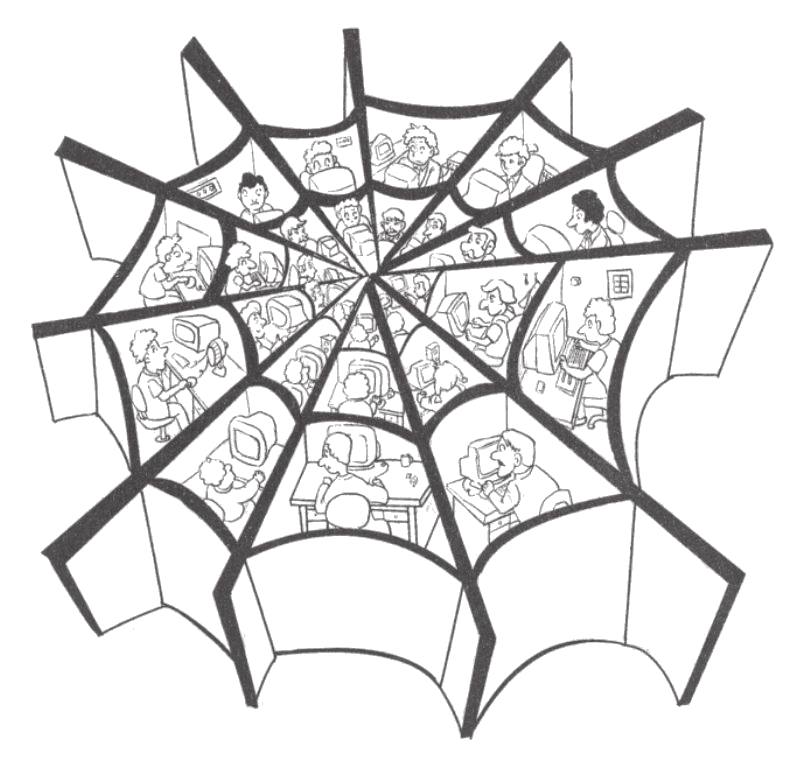
\includegraphics[width=0.32\linewidth]{picture/2009.png}
	\caption*{网络的“近”与“远”}
\end{figure}


